\newpage

\section{Experiments Continued}
\subsection{Hyperparameters}
\label{sec:hyper}
We used 8 H100 GPUs for 340M and 1.3B language modeling experiments. Each model uses AdamW for optimization, with a peak learning rate of $3\times 10^{-4}$. The 340M models are trained using 15 billion tokens and a batch size of 0.5M tokens, while the 1.3B models are trained with 100 billion tokens and a batch size of 2M tokens. We use a cosine learning rate schedule, starting with a warm-up phase of 0.5 billion tokens for the 340M models and 1 billion tokens for the 1.3B models. Both configurations have initial and final learning rates set at $3\times 10^{-5}$. We apply a weight decay of 0.01 and use gradient clipping at a maximum of 1.0. The head dimension of DeltaNet is set to 128, and the kernel size for convolution layers is set at 4. 


\subsection{Synthetic tasks}
\label{sec:regbench}
% \definecolor{color1}{RGB}{116, 184, 22}
% \definecolor{color2}{RGB}{77, 171, 247}
% \definecolor{color3}{RGB}{99, 230, 190}
% \definecolor{color4}{RGB}{132, 94, 247}
% \definecolor{color5}{RGB}{250, 176, 5}

\definecolor{color1}{RGB}{116, 184, 22}
\definecolor{color2}{RGB}{77, 171, 247}
\definecolor{color3}{RGB}{99, 230, 190}
\definecolor{color4}{RGB}{132, 94, 247}
\definecolor{color5}{RGB}{250, 176, 5}

\begin{wrapfigure}{r}{.4\textwidth}
% \vspace{-18mm}
\vspace{-5mm}
	% \begin{figure}[t] %插入图片
		\centering %图片居中
		\resizebox{.4\columnwidth}{!}{  %用于修改图片大小
			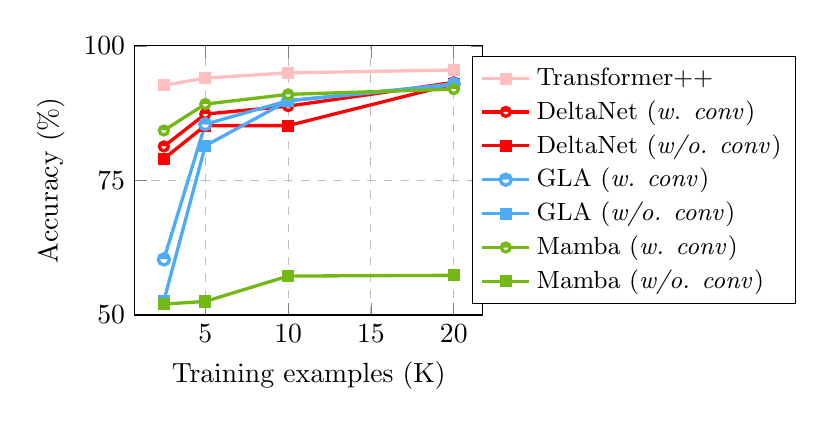
\begin{tikzpicture} %tikz图片
			\scalefont{1} %设置字体大小
			\begin{axis}[
                name=plot2,
                % at={(plot1.south east) },
			sharp plot, %控制线的风格
        title style={align=right},
        % title={Sequence Length: 512, Key-Value Pairs: 64},
			xmode=normal,% 控制坐标轴为线性
%		ymode=log,% 控制坐标轴为对数
			xlabel=Training examples (K), 
   			ylabel=Accuracy ($\%$), 
   %x坐标名
			% ylabel=y, %y坐标名
			width=6cm, height=5cm,  %设置长和宽
			% xmin=0,xmax=20,  % 设置x坐标范围
			ymin=0.5, ymax=1.0,  % 设置y坐标范围
                % x coords={1,2.5,5,10,20,40},
   			ytick={0.50,0.75,1.00}, %指定x轴刻度值。如果为空，则自动设置刻度线。即分割坐标轴,
         yticklabels={50,75,100},
			% ytick, %指定y轴刻度值。如果为空，则自动设置刻度线。即分割坐标轴
			xlabel near ticks, % 设置x坐标名位置靠近折线图
			ylabel near ticks, % 设置y坐标名位置靠近折线图
			ymajorgrids=true, % 启用/禁用 [公式] 轴上刻度线位置上的网格线
			xmajorgrids=true, % 启用/禁用 [公式] 轴上刻度线位置上的网格线
			grid style=dashed, % 设置网格线格式
			legend style={at={(1.9,0.5)},anchor=east, legend cell align=left, font=\small}, 
			]

   		\addplot[very thick, mark=square*, mark options={scale=0.8}, color=pink] plot coordinates {
% (1, 0.5453771134108428)
(2.5, 0.9266456684576904)
(5, 0.9400799353803224)
(10, 0.9497110917689993)
(20, 0.9551300417024798)
% (40, 0.9576954133935113)                    % (40, 0.9375)
% 				% (256,100)
% 				% (512,100)
			};
		\addlegendentry{Transformer++} 

   		\addplot[very thick, mark=halfcircle*, mark options={scale=0.8}, color=red] plot coordinates {
				% (1, 0.5567)
				(2.5, 0.8131)
                    (5, 0.8732)
                    (10, 0.8879)
                    (20, 0.9321)
                    % (40, 0.9375)
				% (256,100)
				% (512,100)
			};
		\addlegendentry{DeltaNet (\textit{w. conv})} 

   		\addplot[very thick, mark=square*, mark options={scale=0.8}, color=red] plot coordinates {
% (1, 0.518813082918104)
(2.5, 0.7903)
(5, 0.8518)
(10, 0.8518)
(20, 0.929)
				% (256,100)
				% (512,100)
			};
		\addlegendentry{DeltaNet (\textit{w/o. conv})} 

   		\addplot[very thick, mark=halfcircle*,  color=color2] plot coordinates {
     % (1, 0.5382)
(2.5, 0.6032)
(5, 0.8543)
(10, 0.898)
(20, 0.929)
% (40, 0.928)
};
		\addlegendentry{GLA (\textit{w. conv})} 
  
   		\addplot[very thick, mark=square*, mark options={scale=0.8}, color=color2] plot coordinates {
% (1, 0.518813082918104)
(2.5, 0.5260845398480718)
(5, 0.8142079368909123)
(10, 0.8979225872754538)
(20, 0.9273920563673214)
};
		\addlegendentry{GLA (\textit{w/o. conv})} 

  %  		\addplot[very thick, mark=circle, mark options={scale=0.8}, color=red] plot coordinates {
		% 		(1, 0.4478)
		% 		(2.5, 0.7903)
  %                   (5, 0.8518)
  %                   (10, 0.8518)
  %                   (20, 0.929)
  %                   (40, 0.926)
		% 		% (256,100)
		% 		% (512,100)
		% 	};
		% \addlegendentry{DeltaNet (\textit{w/o. conv})} 
   		\addplot[very thick,  mark=halfcircle*, mark options={scale=0.8}, color=color1] plot coordinates {
				% (1, 0.6914633107618926)
				(2.5, 0.8427092983245547)
                    (5, 0.8917725303429249)
                    (10, 0.9098144905043047)
                    (20, 0.9195555980008276)
                    % (40, 0.9166100716038952)
				% (256,100)
				% (512,100)
			};
		\addlegendentry{Mamba (\textit{w. conv})} 

   		\addplot[very thick, mark=square*, mark options={scale=0.8}, color=color1] plot coordinates {
% (1, 0.4815)
(2.5, 0.5203)
(5, 0.5252)
(10, 0.5723)
(20, 0.5737)                    % (40, 0.9166100716038952)
				% (256,100)
				% (512,100)
			};
		\addlegendentry{Mamba (\textit{w/o. conv})} 


			\end{axis}
			\end{tikzpicture}
  }
    \vspace{-6mm}
		% \caption{The x-axis is the model dimension and the y-axis is accuracy on MQAR.} 
		\caption{Accuracy (\%) on RegBench.} 
		\label{fig:regbench} 
    \vspace{-6mm}
	% \end{figure}/
\end{wrapfigure}

We additional conduct experiments on RegBench~\citep{akyurek2024context},  a synthetic data set designed to assess the in-context language learning capability of different model architectures. Each input sequence in this benchmark consists of 10 to 20 strings drawn from a distinct language defined by a  probabilistic finite automaton (PFA), so that a model needs to infer the underlying language from the context on the fly.  During testing, a model is evaluated on
predicting the next token of testing sequences generated from held-out PFAs.  Here again we find that DeltaNet performs strongly compared to baselines, as shown in  Figure \ref{fig:regbench}. 


\section{Method Continued}
\subsection{WY representation derivation}
To reduce notational clutter, we discuss only the first chunk here.

We first show $\rmP_n = \rmI - \sum_{t=1}^n \vw_t\vk_t^{\intercal}$ by induction,
\begin{align*}
\rmP_n &= \prod_{t=1}^n(\rmI - \beta_t \vk_t \vk_t^\intercal)     \\
&= \rmP_{n-1} (\rmI - \beta_n \vk_n \vk_n^\intercal)  \\
&=  (\rmI - \sum_{t=1}^{n-1} \vw_t \vk_t^\intercal)  (\rmI - \beta_n \vk_n \vk_n^\intercal) \\
&=  \rmI - \sum_{t=1}^{n-1} \vw_t \vk_t^\intercal - \beta_n \vk_n \vk_n^\intercal + (\sum_{t=1}^{n-1} \vw_t \vk_t^\intercal) \beta_n \vk_n \vk_n^\intercal \\
&= \rmI - \sum_{t=1}^{n-1} \vw_t \vk_t^\intercal  - \underbrace{\left(\beta_n \vk_n - \beta_n \sum_{t=1}^{n-1} \left(\vw_t (\vk_t^\intercal\vk_n)\right) \right)}_{\vw_n}\vk_n^\intercal \\
&= \rmI - \sum_{t=1}^n \vw_t\vk_t^{\intercal}
\end{align*}

Similarly, we show $\rmS_n = \sum_{t=1}^{n} \vu_t \vk_n^\intercal$ by induction, 
\begin{align*}
    \rmS_n & = \rmS_{n-1} (\rmI - \beta_n \vk_n\vk_n^\intercal) + \beta_n \vv_n  \vk_n^\intercal \\
    & =  \left(\sum_{t=1}^{n-1} \vu_{t}\vk_{t}^\intercal\right) (\rmI - \beta_n \vk_n\vk_n^\intercal )  + \beta_n \vv_n  \vk_n^\intercal \\
    &= \sum_{t=1}^{n-1} \vu_{t}\vk_{t}^\intercal - \left(\sum_{t=1}^{n-1} \vu_{t}\vk_{t}^\intercal\right) \beta_n \vk_n \vk_n^\intercal + \beta_n \vv_n \vk_n^\intercal \\
    &= \sum_{t=1}^{n-1} \vu_{t}\vk_{t}^\intercal + \underbrace{\left(\beta_n \vv_n - \beta_n\sum_{t=1}^{n-1} \vu_t \left(\vk_t^{\intercal} \vk_n \right)  \right)}_{\vu_n} \vk_n^{\intercal} \\
    &= \sum_{t=1}^{n} \vu_t \vk_n^\intercal
    % & =  \rmW_{t-1} \rmY_{t-1}^\intercal - \rmW_{t-1} \rmY_{t-1}^\intercal \beta_t \vk_t\vk_t^\intercal   + \beta_t \vv_t  \vk_t^\intercal \\
    % & = [\rmW_{t-1}; \beta_t\vv_t- \beta_t \left(\rmW_{t-1} \left(\rmY_{t-1}^\intercal  \vk_t\right)\right)] [\rmY_{t-1}; \vk_t]^\intercal  
    \label{eq:wy_s_final}
\end{align*}

\subsection{UT transform derivation} 


\label{appendix:ut_transform}

Here we provide a detailed derivation of the UT transform used in \S\ref{sec:chunk_deltanet}. Specifically, we show that the matrix formulation using the UT transform (Equations \ref{eq:inverse} and \ref{eq:wu=akv} in the main text) is equivalent to the recursive update equations (Equation \ref{eq:wy-u}).

We begin with the recursive formulation for computing $\vw_{[t]}^r$ and $\vu_{[t]}^r$ as given in Equation \ref{eq:wy-u}:
\begin{align*}
    \vw_{[t]}^r &= \beta_{[t]}^r \left(\vk_{[t]}^r -  \sum_{i=1}^{r-1} \vw_{[t]}^i (\vk_{[t]}^{i\intercal}\vk_{[t]}^r)  \right) \\
    \vu_{[t]}^r &= \beta_{[t]}^r \left(\vv_{[t]}^r -  \sum_{i=1}^{r-1} \vu_{[t]}^i (\vk_{[t]}^{i\intercal}\vk_{[t]}^r)  \right)
\end{align*}

Our goal is to show that these recursive updates can be rewritten in matrix form using the UT transform:
\begin{align*}
    \rmT_{[t]} &= \left(\rmI + \operatorname{tril}(\operatorname{diag}(\beta_{[t]})\rmK_{[t]} \rmK_{[t]}^\intercal,-1)\right)^{-1}\operatorname{diag}\left(\beta_{[t]}\right) \\
    \rmW_{[t]} &= \rmT_{[t]} \rmK_{[t]} \\
    \rmU_{[t]} &= \rmT_{[t]} \rmV_{[t]}
\end{align*}

First, let us consider the computation of $\vw_{[t]}^r$. For any row $r$, we can write:
\begin{equation*}
    \rmW_{[t]}[r,:] = \beta_{[t]}^r \rmK_{[t]}[r,:] - \beta_{[t]}^r \sum_{i=1}^{r-1} \rmW_{[t]}[i,:] (\rmK_{[t]}[i,:]\rmK_{[t]}[r,:]^\intercal)
\end{equation*}

This system of equations can be written in matrix form. Let us define:
\begin{equation*}
    \rmB_{[t]} = \operatorname{diag}(\beta_{[t]})
\end{equation*}
\begin{equation*}
    \rmL_{[t]} = \operatorname{tril}(\rmB_{[t]}\rmK_{[t]}\rmK_{[t]}^\intercal, -1)
\end{equation*}

Then the system becomes:
\begin{equation*}
    \rmW_{[t]} + \rmL_{[t]}\rmW_{[t]} = \rmB_{[t]}\rmK_{[t]}
\end{equation*}

Thus, we can solve for $\rmW_{[t]}$:
\begin{equation*}
    \rmW_{[t]} = (\rmI + \rmL_{[t]})^{-1}\rmB_{[t]}\rmK_{[t]} = \rmT_{[t]}\rmK_{[t]}
\end{equation*}

where
\begin{equation*}
    \rmT_{[t]} = (\rmI + \rmL_{[t]})^{-1}\rmB_{[t]}
\end{equation*}


The same derivation applies for $\rmU_{[t]}$ by replacing $\rmK_{[t]}$ with $\rmV_{[t]}$ in the final step, yielding:
\begin{equation}
    \rmU_{[t]} = \rmT_{[t]}\rmV_{[t]}
\end{equation}




\section{Related Work Continued}
\label{app:related}
\paragraph{Chunkwise linear attention.} \citet{hua_transformer_2022} first proposed chunkwise form for linear attention; however, they used a hybrid linear and nonlinear attention model similar to \citet{munkhdalai2024leave}.  It is possible to adapt their algorithm to compute the \emph{exact} output of the pure linear attention, as shown in \citet{sun2023retentive} and \citet{yang_gated_2023}. The chunkwise linear attention algorithm has also been independently discovered in several works \cite{sun2023retentive, polysketch, mamba2}.  \citet{yang_gated_2023} and \citet{lightning2} discuss I/O-aware hardware optimization for chunkwise linear attention and \citet{Sun2024LinearAS} make generalization to multi-node distributed training. Inspired by the chunkwise form, we propose a new algorithm for hardware-efficient DeltaNet training, significantly improving the training efficiency and allowing for large-scale experiments. 

\paragraph{Hybrid models.}  Linear recurrent models - including state-space models \cite{s4, s5, gu_mamba_2023, pretrain_wo_attn}, gated linear RNNs \cite{parallel-martin, HGRN}, and linear attention mechanisms \cite{katharopoulos_transformers_2020, yang_gated_2023} - have demonstrated remarkable potential as alternatives to traditional softmax attention across diverse domains \cite{Yan2023DiffusionMW, Zhu2024DiGSA, Liao2024ViGLV, Zhu2024VisionME, Wang2024GraphMambaTL, Schiff2024CaduceusBE}. Given their complementary strengths, recent research has increasingly focused on developing hybrid architectures that combine linear recurrent layers with local chunk attention \cite{Ma2022MegaMA, zhang-etal-2023-efficient-long, Fathi2023BlockStateT, Ma2024MegalodonEL, munkhdalai2024leave} or sliding window attention \cite{zhang-etal-2023-efficient-long, arora_simple_2024, de_griffin_2024, ren2024samba} or global attention \cite{lei_when_2021, Lei2022SimpleRI, huang_encoding_2022, fu_hungry_2023, Lieber2024JambaAH, Park2024CanML, Sun2024YouOC}.  \citet{poli_mechanistic_2024} systematically study the scaling law of hybrid models. We similarly show that combining DeltaNet with classic attention is an effective strategy.



\paragraph{Householder matrices.}
Householder matrices, known for preserving norms, are a type of orthogonal matrix extensively used in machine learning \cite{mathiasen_faster_nodate,mhammedi_efficient_2017,zhang_stabilizing_2018,tomczak_improving_2017,qin_linearized_2023,berg_sylvester_2019}. These matrices allow for  efficient computation of inverses and their Jacobian determinant of one, making them particularly suitable for applications in normalizing flows \cite{mathiasen_faster_nodate,berg_sylvester_2019}. Notably, \citet{mathiasen_faster_nodate} and  \citet{Mathiasen2020WhatIN} developed a chunkwise fast algorithm for computing the cumulative product of Householder matrices for normalizing flows, leveraging the WY representation. Our approach, while sharing the same high-level concept, tackles a different problem and is arguably more general.

There has also been significant interest in using orthogonal matrices to parameterize the transition matrices of RNNs \cite{mhammedi_efficient_2017,jing_gated_2019,vorontsov_orthogonality_2016,helfrich_orthogonal_2018} for mitigating vanishing gradients.  \citet{mhammedi_efficient_2017} use the WY representation to reduce the memory footprint when training nonlinear RNNs with Householder transition matrices.

% In numerical algebra, householder matrix plays a important role in .  UT transform 



\newpage
\section{Pseudo code}
\input{tables/chunk_code2}




% \newpage
% \mbox{~}

% \section*{NeurIPS Paper Checklist}

% %%% BEGIN INSTRUCTIONS %%%
% The checklist is designed to encourage best practices for responsible machine learning research, addressing issues of reproducibility, transparency, research ethics, and societal impact. Do not remove the checklist: {\bf The papers not including the checklist will be desk rejected.} The checklist should follow the references and follow the (optional) supplemental material.  The checklist does NOT count towards the page
% limit.

% Please read the checklist guidelines carefully for information on how to answer these questions. For each question in the checklist:
% \begin{itemize}
%   \item You should answer \answerYes{}, \answerNo{}, or \answerNA{}.
%   \item \answerNA{} means either that the question is Not Applicable for that particular paper or the relevant information is Not Available.
%   \item Please provide a short (1–2 sentence) justification right after your answer (even for NA).
%         % \item {\bf The papers not including the checklist will be desk rejected.}
% \end{itemize}

% {\bf The checklist answers are an integral part of your paper submission.} They are visible to the reviewers, area chairs, senior area chairs, and ethics reviewers. You will be asked to also include it (after eventual revisions) with the final version of your paper, and its final version will be published with the paper.

% The reviewers of your paper will be asked to use the checklist as one of the factors in their evaluation. While "\answerYes{}" is generally preferable to "\answerNo{}", it is perfectly acceptable to answer "\answerNo{}" provided a proper justification is given (e.g., "error bars are not reported because it would be too computationally expensive" or "we were unable to find the license for the dataset we used"). In general, answering "\answerNo{}" or "\answerNA{}" is not grounds for rejection. While the questions are phrased in a binary way, we acknowledge that the true answer is often more nuanced, so please just use your best judgment and write a justification to elaborate. All supporting evidence can appear either in the main paper or the supplemental material, provided in appendix. If you answer \answerYes{} to a question, in the justification please point to the section(s) where related material for the question can be found.

% IMPORTANT, please:
% \begin{itemize}
%   \item {\bf Delete this instruction block, but keep the section heading ``NeurIPS paper checklist"},
%   \item  {\bf Keep the checklist subsection headings, questions/answers and guidelines below.}
%   \item {\bf Do not modify the questions and only use the provided macros for your answers}.
% \end{itemize}


% %% END INSTRUCTIONS %%%


% \begin{enumerate}

%       \item {\bf Claims}
%       \item[] Question: Do the main claims made in the abstract and introduction accurately reflect the paper's contributions and scope?
%       \item[] Answer: \answerYes{} % Replace by \answerYes{}, \answerNo{}, or \answerNA{}.
%       \item[] Justification: This paper's contributions and scope are reflected in abstract and introduction part clearly.
%       \item[] Guidelines:
%             \begin{itemize}
%                   \item The answer NA means that the abstract and introduction do not include the claims made in the paper.
%                   \item The abstract and/or introduction should clearly state the claims made, including the contributions made in the paper and important assumptions and limitations. A No or NA answer to this question will not be perceived well by the reviewers.
%                   \item The claims made should match theoretical and experimental results, and reflect how much the results can be expected to generalize to other settings.
%                   \item It is fine to include aspirational goals as motivation as long as it is clear that these goals are not attained by the paper.
%             \end{itemize}

%       \item {\bf Limitations}
%       \item[] Question: Does the paper discuss the limitations of the work performed by the authors?
%       \item[] Answer: \answerYes{} % Replace by \answerYes{}, \answerNo{}, or \answerNA{}.
%       \item[] Justification: We discuss the limitations of this work in \S\ref{sec:limitation}.
%       \item[] Guidelines:
%             \begin{itemize}
%                   \item The answer NA means that the paper has no limitation while the answer No means that the paper has limitations, but those are not discussed in the paper.
%                   \item The authors are encouraged to create a separate "Limitations" section in their paper.
%                   \item The paper should point out any strong assumptions and how robust the results are to violations of these assumptions (e.g., independence assumptions, noiseless settings, model well-specification, asymptotic approximations only holding locally). The authors should reflect on how these assumptions might be violated in practice and what the implications would be.
%                   \item The authors should reflect on the scope of the claims made, e.g., if the approach was only tested on a few datasets or with a few runs. In general, empirical results often depend on implicit assumptions, which should be articulated.
%                   \item The authors should reflect on the factors that influence the performance of the approach. For example, a facial recognition algorithm may perform poorly when image resolution is low or images are taken in low lighting. Or a speech-to-text system might not be used reliably to provide closed captions for online lectures because it fails to handle technical jargon.
%                   \item The authors should discuss the computational efficiency of the proposed algorithms and how they scale with dataset size.
%                   \item If applicable, the authors should discuss possible limitations of their approach to address problems of privacy and fairness.
%                   \item While the authors might fear that complete honesty about limitations might be used by reviewers as grounds for rejection, a worse outcome might be that reviewers discover limitations that aren't acknowledged in the paper. The authors should use their best judgment and recognize that individual actions in favor of transparency play an important role in developing norms that preserve the integrity of the community. Reviewers will be specifically instructed to not penalize honesty concerning limitations.
%             \end{itemize}

%       \item {\bf Theory Assumptions and Proofs}
%       \item[] Question: For each theoretical result, does the paper provide the full set of assumptions and a complete (and correct) proof?
%       \item[] Answer: \answerNA{} % Replace by \answerYes{}, \answerNo{}, or \answerNA{}.
%       \item[] Justification: This paper does not include theoretical results that require a full proof.
%       \item[] Guidelines:
%             \begin{itemize}
%                   \item The answer NA means that the paper does not include theoretical results.
%                   \item All the theorems, formulas, and proofs in the paper should be numbered and cross-referenced.
%                   \item All assumptions should be clearly stated or referenced in the statement of any theorems.
%                   \item The proofs can either appear in the main paper or the supplemental material, but if they appear in the supplemental material, the authors are encouraged to provide a short proof sketch to provide intuition.
%                   \item Inversely, any informal proof provided in the core of the paper should be complemented by formal proofs provided in appendix or supplemental material.
%                   \item Theorems and Lemmas that the proof relies upon should be properly referenced.
%             \end{itemize}

%       \item {\bf Experimental Result Reproducibility}
%       \item[] Question: Does the paper fully disclose all the information needed to reproduce the main experimental results of the paper to the extent that it affects the main claims and/or conclusions of the paper (regardless of whether the code and data are provided or not)?
%       \item[] Answer: \answerYes{} % Replace by \answerYes{}, \answerNo{}, or \answerNA{}.
%       \item[] Justification: The paper provides sufficient details on hyperparameters and training procedures in \S\ref{sec:hyper} to reproduce the results supporting its main conclusions.
%       \item[] Guidelines:
%             \begin{itemize}
%                   \item The answer NA means that the paper does not include experiments.
%                   \item If the paper includes experiments, a No answer to this question will not be perceived well by the reviewers: Making the paper reproducible is important, regardless of whether the code and data are provided or not.
%                   \item If the contribution is a dataset and/or model, the authors should describe the steps taken to make their results reproducible or verifiable.
%                   \item Depending on the contribution, reproducibility can be accomplished in various ways. For example, if the contribution is a novel architecture, describing the architecture fully might suffice, or if the contribution is a specific model and empirical evaluation, it may be necessary to either make it possible for others to replicate the model with the same dataset, or provide access to the model. In general. releasing code and data is often one good way to accomplish this, but reproducibility can also be provided via detailed instructions for how to replicate the results, access to a hosted model (e.g., in the case of a large language model), releasing of a model checkpoint, or other means that are appropriate to the research performed.
%                   \item While NeurIPS does not require releasing code, the conference does require all submissions to provide some reasonable avenue for reproducibility, which may depend on the nature of the contribution. For example
%                         \begin{enumerate}
%                               \item If the contribution is primarily a new algorithm, the paper should make it clear how to reproduce that algorithm.
%                               \item If the contribution is primarily a new model architecture, the paper should describe the architecture clearly and fully.
%                               \item If the contribution is a new model (e.g., a large language model), then there should either be a way to access this model for reproducing the results or a way to reproduce the model (e.g., with an open-source dataset or instructions for how to construct the dataset).
%                               \item We recognize that reproducibility may be tricky in some cases, in which case authors are welcome to describe the particular way they provide for reproducibility. In the case of closed-source models, it may be that access to the model is limited in some way (e.g., to registered users), but it should be possible for other researchers to have some path to reproducing or verifying the results.
%                         \end{enumerate}
%             \end{itemize}


%       \item {\bf Open access to data and code}
%       \item[] Question: Does the paper provide open access to the data and code, with sufficient instructions to faithfully reproduce the main experimental results, as described in supplemental material?
%       \item[] Answer: \answerYes{} % Replace by \answerYes{}, \answerNo{}, or \answerNA{}.
%       \item[] Justification: Our code is publicly available at \url{https://github.com/sustcsonglin/flash-linear-attention}. Our primary training corpus is Slimpajama, an open-source dataset.
%       \item[] Guidelines:
%             \begin{itemize}
%                   \item The answer NA means that paper does not include experiments requiring code.
%                   \item Please see the NeurIPS code and data submission guidelines (\url{https://nips.cc/public/guides/CodeSubmissionPolicy}) for more details.
%                   \item While we encourage the release of code and data, we understand that this might not be possible, so “No” is an acceptable answer. Papers cannot be rejected simply for not including code, unless this is central to the contribution (e.g., for a new open-source benchmark).
%                   \item The instructions should contain the exact command and environment needed to run to reproduce the results. See the NeurIPS code and data submission guidelines (\url{https://nips.cc/public/guides/CodeSubmissionPolicy}) for more details.
%                   \item The authors should provide instructions on data access and preparation, including how to access the raw data, preprocessed data, intermediate data, and generated data, etc.
%                   \item The authors should provide scripts to reproduce all experimental results for the new proposed method and baselines. If only a subset of experiments are reproducible, they should state which ones are omitted from the script and why.
%                   \item At submission time, to preserve anonymity, the authors should release anonymized versions (if applicable).
%                   \item Providing as much information as possible in supplemental material (appended to the paper) is recommended, but including URLs to data and code is permitted.
%             \end{itemize}


%       \item {\bf Experimental Setting/Details}
%       \item[] Question: Does the paper specify all the training and test details (e.g., data splits, hyperparameters, how they were chosen, type of optimizer, etc.) necessary to understand the results?
%       \item[] Answer: \answerYes{} % Replace by \answerYes{}, \answerNo{}, or \answerNA{}.
%       \item[] Justification: We have detailed all the training and evaluation settings before the main results in the experimental part.
%       \item[] Guidelines:
%             \begin{itemize}
%                   \item The answer NA means that the paper does not include experiments.
%                   \item The experimental setting should be presented in the core of the paper to a level of detail that is necessary to appreciate the results and make sense of them.
%                   \item The full details can be provided either with the code, in appendix, or as supplemental material.
%             \end{itemize}

%       \item {\bf Experiment Statistical Significance}
%       \item[] Question: Does the paper report error bars suitably and correctly defined or other appropriate information about the statistical significance of the experiments?
%       \item[] Answer: \answerNo{} % Replace by \answerYes{}, \answerNo{}, or \answerNA{}.
%       \item[] Justification: We do not have enough resources to obtain error bars as running the experiments multiple times is computationally expensive due to the large model size.
%       \item[] Guidelines:
%             \begin{itemize}
%                   \item The answer NA means that the paper does not include experiments.
%                   \item The authors should answer "Yes" if the results are accompanied by error bars, confidence intervals, or statistical significance tests, at least for the experiments that support the main claims of the paper.
%                   \item The factors of variability that the error bars are capturing should be clearly stated (for example, train/test split, initialization, random drawing of some parameter, or overall run with given experimental conditions).
%                   \item The method for calculating the error bars should be explained (closed form formula, call to a library function, bootstrap, etc.)
%                   \item The assumptions made should be given (e.g., Normally distributed errors).
%                   \item It should be clear whether the error bar is the standard deviation or the standard error of the mean.
%                   \item It is OK to report 1-sigma error bars, but one should state it. The authors should preferably report a 2-sigma error bar than state that they have a 96\% CI, if the hypothesis of Normality of errors is not verified.
%                   \item For asymmetric distributions, the authors should be careful not to show in tables or figures symmetric error bars that would yield results that are out of range (e.g. negative error rates).
%                   \item If error bars are reported in tables or plots, The authors should explain in the text how they were calculated and reference the corresponding figures or tables in the text.
%             \end{itemize}

%       \item {\bf Experiments Compute Resources}
%       \item[] Question: For each experiment, does the paper provide sufficient information on the computer resources (type of compute workers, memory, time of execution) needed to reproduce the experiments?
%       \item[] Answer: \answerYes{} % Replace by \answerYes{}, \answerNo{}, or \answerNA{}.
%       \item[] Justification: We provide information of GPU type and number of GPUs used for running our experiments.
%       \item[] Guidelines:
%             \begin{itemize}
%                   \item The answer NA means that the paper does not include experiments.
%                   \item The paper should indicate the type of compute workers CPU or GPU, internal cluster, or cloud provider, including relevant memory and storage.
%                   \item The paper should provide the amount of compute required for each of the individual experimental runs as well as estimate the total compute.
%                   \item The paper should disclose whether the full research project required more compute than the experiments reported in the paper (e.g., preliminary or failed experiments that didn't make it into the paper).
%             \end{itemize}

%       \item {\bf Code Of Ethics}
%       \item[] Question: Does the research conducted in the paper conform, in every respect, with the NeurIPS Code of Ethics \url{https://neurips.cc/public/EthicsGuidelines}?
%       \item[] Answer: \answerYes{} % Replace by \answerYes{}, \answerNo{}, or \answerNA{}.
%       \item[] Justification: This work follows the NeurIPS Code of Ethics.
%       \item[] Guidelines:
%             \begin{itemize}
%                   \item The answer NA means that the authors have not reviewed the NeurIPS Code of Ethics.
%                   \item If the authors answer No, they should explain the special circumstances that require a deviation from the Code of Ethics.
%                   \item The authors should make sure to preserve anonymity (e.g., if there is a special consideration due to laws or regulations in their jurisdiction).
%             \end{itemize}


%       \item {\bf Broader Impacts}
%       \item[] Question: Does the paper discuss both potential positive societal impacts and negative societal impacts of the work performed?
%       \item[] Answer: \answerNA{} % Replace by \answerYes{}, \answerNo{}, or \answerNA{}.
%       \item[] Justification: We foresee no potential societal impact of this work.
%       \item[] Guidelines:
%             \begin{itemize}
%                   \item The answer NA means that there is no societal impact of the work performed.
%                   \item If the authors answer NA or No, they should explain why their work has no societal impact or why the paper does not address societal impact.
%                   \item Examples of negative societal impacts include potential malicious or unintended uses (e.g., disinformation, generating fake profiles, surveillance), fairness considerations (e.g., deployment of technologies that could make decisions that unfairly impact specific groups), privacy considerations, and security considerations.
%                   \item The conference expects that many papers will be foundational research and not tied to particular applications, let alone deployments. However, if there is a direct path to any negative applications, the authors should point it out. For example, it is legitimate to point out that an improvement in the quality of generative models could be used to generate deepfakes for disinformation. On the other hand, it is not needed to point out that a generic algorithm for optimizing neural networks could enable people to train models that generate Deepfakes faster.
%                   \item The authors should consider possible harms that could arise when the technology is being used as intended and functioning correctly, harms that could arise when the technology is being used as intended but gives incorrect results, and harms following from (intentional or unintentional) misuse of the technology.
%                   \item If there are negative societal impacts, the authors could also discuss possible mitigation strategies (e.g., gated release of models, providing defenses in addition to attacks, mechanisms for monitoring misuse, mechanisms to monitor how a system learns from feedback over time, improving the efficiency and accessibility of ML).
%             \end{itemize}

%       \item {\bf Safeguards}
%       \item[] Question: Does the paper describe safeguards that have been put in place for responsible release of data or models that have a high risk for misuse (e.g., pretrained language models, image generators, or scraped datasets)?
%       \item[] Answer: \answerNA{} % Replace by \answerYes{}, \answerNo{}, or \answerNA{}.
%       \item[] Justification: We foresee no such risks posed by this work.
%       \item[] Guidelines:
%             \begin{itemize}
%                   \item The answer NA means that the paper poses no such risks.
%                   \item Released models that have a high risk for misuse or dual-use should be released with necessary safeguards to allow for controlled use of the model, for example by requiring that users adhere to usage guidelines or restrictions to access the model or implementing safety filters.
%                   \item Datasets that have been scraped from the Internet could pose safety risks. The authors should describe how they avoided releasing unsafe images.
%                   \item We recognize that providing effective safeguards is challenging, and many papers do not require this, but we encourage authors to take this into account and make a best faith effort.
%             \end{itemize}

%       \item {\bf Licenses for existing assets}
%       \item[] Question: Are the creators or original owners of assets (e.g., code, data, models), used in the paper, properly credited and are the license and terms of use explicitly mentioned and properly respected?
%       \item[] Answer: \answerYes{} % Replace by \answerYes{}, \answerNo{}, or \answerNA{}.
%       \item[] Justification: All of the datasets we use are publicly available at huggingface site, and we have properly cited all the training and evaluation datasets we used.
%       \item[] Guidelines:
%             \begin{itemize}
%                   \item The answer NA means that the paper does not use existing assets.
%                   \item The authors should cite the original paper that produced the code package or dataset.
%                   \item The authors should state which version of the asset is used and, if possible, include a URL.
%                   \item The name of the license (e.g., CC-BY 4.0) should be included for each asset.
%                   \item For scraped data from a particular source (e.g., website), the copyright and terms of service of that source should be provided.
%                   \item If assets are released, the license, copyright information, and terms of use in the package should be provided. For popular datasets, \url{paperswithcode.com/datasets} has curated licenses for some datasets. Their licensing guide can help determine the license of a dataset.
%                   \item For existing datasets that are re-packaged, both the original license and the license of the derived asset (if it has changed) should be provided.
%                   \item If this information is not available online, the authors are encouraged to reach out to the asset's creators.
%             \end{itemize}

%       \item {\bf New Assets}
%       \item[] Question: Are new assets introduced in the paper well documented and is the documentation provided alongside the assets?
%       \item[] Answer: \answerNA{} % Replace by \answerYes{}, \answerNo{}, or \answerNA{}.
%       \item[] Justification: This work does not release new assets.
%       \item[] Guidelines:
%             \begin{itemize}
%                   \item The answer NA means that the paper does not release new assets.
%                   \item Researchers should communicate the details of the dataset/code/model as part of their submissions via structured templates. This includes details about training, license, limitations, etc.
%                   \item The paper should discuss whether and how consent was obtained from people whose asset is used.
%                   \item At submission time, remember to anonymize your assets (if applicable). You can either create an anonymized URL or include an anonymized zip file.
%             \end{itemize}

%       \item {\bf Crowdsourcing and Research with Human Subjects}
%       \item[] Question: For crowdsourcing experiments and research with human subjects, does the paper include the full text of instructions given to participants and screenshots, if applicable, as well as details about compensation (if any)?
%       \item[] Answer: \answerNA{} % Replace by \answerYes{}, \answerNo{}, or \answerNA{}.
%       \item[] Justification: This work does not involve crowdsourcing nor research with human subjects.
%       \item[] Guidelines:
%             \begin{itemize}
%                   \item The answer NA means that the paper does not involve crowdsourcing nor research with human subjects.
%                   \item Including this information in the supplemental material is fine, but if the main contribution of the paper involves human subjects, then as much detail as possible should be included in the main paper.
%                   \item According to the NeurIPS Code of Ethics, workers involved in data collection, curation, or other labor should be paid at least the minimum wage in the country of the data collector.
%             \end{itemize}

%       \item {\bf Institutional Review Board (IRB) Approvals or Equivalent for Research with Human Subjects}
%       \item[] Question: Does the paper describe potential risks incurred by study participants, whether such risks were disclosed to the subjects, and whether Institutional Review Board (IRB) approvals (or an equivalent approval/review based on the requirements of your country or institution) were obtained?
%       \item[] Answer: \answerNA{} % Replace by \answerYes{}, \answerNo{}, or \answerNA{}.
%       \item[] Justification: This work does not involve crowdsourcing nor research with human subjects.
%       \item[] Guidelines:
%             \begin{itemize}
%                   \item The answer NA means that the paper does not involve crowdsourcing nor research with human subjects.
%                   \item Depending on the country in which research is conducted, IRB approval (or equivalent) may be required for any human subjects research. If you obtained IRB approval, you should clearly state this in the paper.
%                   \item We recognize that the procedures for this may vary significantly between institutions and locations, and we expect authors to adhere to the NeurIPS Code of Ethics and the guidelines for their institution.
%                   \item For initial submissions, do not include any information that would break anonymity (if applicable), such as the institution conducting the review.
%             \end{itemize}

% \end{enumerate}